\section*{Neural Networks}
There are several categories of statistical algorithms for data analysis within machine learning.
Amongst them are neural networks, which have for the last decade exponentially been used
within industry and academia for a number of usecases. From image analysis to weather prediction,
these models are used extensively. \par
Neural networks, or feed forward neural networks (FFNN), are based on a few principles.
First, the data is feeded forward through the network. The end output is evaluated in some fashion, 
and corrections are then back propagated through the network, updating the weights and biases. 
This "training" is done until a sufficient threshold is met. A general layout of a neural network is displayed in
figure \ref{fig:nndiagram}.

\begin{figure}
    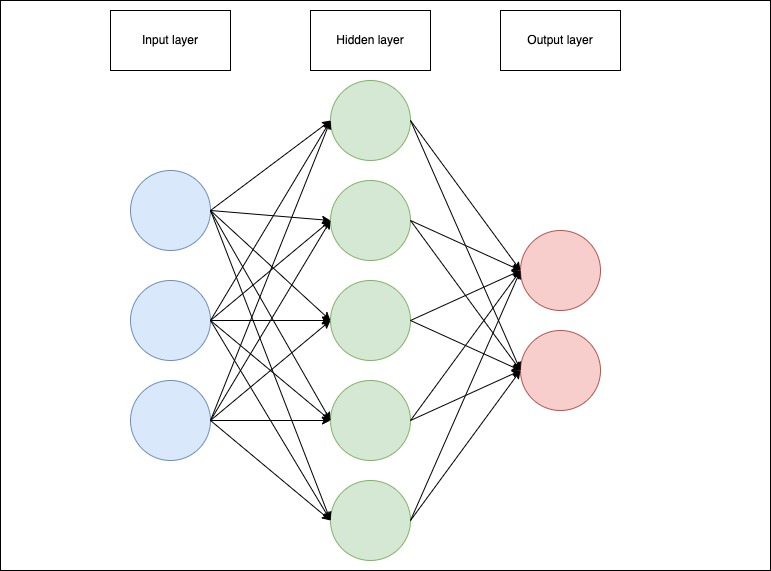
\includegraphics[width=\linewidth]{Figures/Machinelearning/nn_diagram.jpeg}
    \caption{Simple neural network diagram drawm using Draw.io. Here the blue dots are the input layer, the green dots are a hidden layer, and the red dots are the output layer. The arrows shows the connections between each node. }
    \label{fig:nndiagram}
\end{figure}

The input layer has the same shape of the dataset one uses to train or predict on, with one node for each feature in the dataset.
The next layer is the hidden layers. For a given network, the amount of hidden layers can be tuned, as well as the number of 
nodes per layer. Finally, the last hidden layer is connected to the ouput layer, which is determined by the aim of the problem. 
In the case of figure \ref{fig:nndiagram}, this neural network would represent a binary classification problem, in other words, two categories. 
The nodes in the network interacts through so called weights $w$ and biases $b$. These are known as tunable parameters, 
which needs to be trained on the dataset before any prediction can be made. 


\subsection*{Backpropagation}

\subsection*{Feed forwarding}